%%
%% ****** Generated 24.03.23 by LJM TeX-constructor******
%%
\documentclass{article}

\usepackage{amssymb}
\usepackage{amsfonts}
\usepackage[tbtags]{amsmath}
\usepackage{amscd}
\usepackage{amsthm}			% Продвинутая математика
\usepackage{mathtext}
\usepackage{cmap}
\usepackage[T2A]{fontenc}
\usepackage[utf8]{inputenc}			% cp1251
\usepackage[english, russian]{babel}
%\usepackage{literat}
\usepackage{pifont}
\usepackage{bm}
\usepackage{array}			% Ширина столбиков в массиве
\usepackage{dcolumn}
\usepackage{hhline}
\usepackage{multirow}
\usepackage{graphicx}
\usepackage{rotating}
\usepackage{calc}
\usepackage{tabularx}
\usepackage{afterpage}
\usepackage{ifthen}
\usepackage{caption2}
\usepackage{substr}
\usepackage[mathscr]{eucal}  %% My addition
\usepackage{mathrsfs}        %% My addition
\usepackage{hypbmsec}        %% My addition
\usepackage{latexsym}        %% My addition
\usepackage{xypic}           %% My addition
\RequirePackage{soul}
\RequirePackage{verbatim}    %% My addition
\RequirePackage{chapterbib}
\RequirePackage{enumerate}


\usepackage[shortcuts]{extdash}
\usepackage{ragged2e}
\usepackage{etoolbox}
\usepackage{lipsum}

%\usepackage{flafter}
\usepackage[section,above,below]{placeins}

\usepackage{indentfirst}
\usepackage[a4paper, top=20mm, left=30mm, right=20mm, bottom=25mm]{geometry}


\setcounter{page}{1}

\begin{document}
\title{Influence of weight coefficients on the solution of the inverse problem} % for running heads
\author{Kosyakov} % for running heads
\author{Legostaev}

%\noaffiliation % If the author does not specify a place of work.

%\firstcollaboration{(Submitted by ) } % Add if you know submitter.
%\lastcollaboration{ }


\begin{abstract} % You shouldn't use formulas and citations in the abstract.
In the oil industry, there is a noticeable tendency to proxy modeling of various levels of complexity to perform operational predictive calculations, in particular, machine learning methods that are actively developing in the context of digitalization and intellectualization of production processes. In this paper, using the example of a synthetic oil reservoir model development element, we present an approach to the joint use of a physically meaningful fluid flow model and machine learning methods for solving adaptation and prediction problems. A feature of the considered synthetic model is the presence of a pronounced zonal inhomogeneity of the permeability field. Within the framework of the proposed approach, a single-phase filtration model, simplified in comparison with the original formulation, was used, which was history-matched by restoring the field of reservoir filtration parameters using a network of radial basis functions. Based on the reconstructed field, the connection coefficients between the wells were calculated, which qualitatively and quantitatively correspond to the true well connection. The next step was to train the recurrent neural network in order to predict the water cut of the produced fluid. The use of a recurrent neural network made it possible to reproduce the characteristic non-monotonic behavior of the water cut of the produced fluid, caused by non-stationary modes of operation of injection and production wells. A combination of the presented models makes it possible to predict the volume of the produced fluid and its phase composition. To assess the predictive properties of the models, the actual data set was divided into training and test intervals.
\end{abstract}

\textbf{Keywords}:flow through porous medium, reservoir mathematical simulation, inverse problem, adjoint problem, machine learning, radial basis functions, recurrent neural networks % Include keywords separeted by comma.

\maketitle

% Text of article starts here.

Адаптация модели на историю происходит за счет настройки фильтрационных параметров пласта. Предлагаемый подход предполагает использование постоянного во времени поля общей подвижности, которое наилучшим образом позволит описать историю разработки. Однако, при вытеснении нефти водой происходит постепенное изменение фазового состава жидкости в пласте, что приводит к изменению общей подвижности. Таким образом, решение обратной задачи сводится к определению некоторого эффективного поля общей подвижности, которое так же (далее) используется для прогнозных расчетов.

\section{INTRODUCTION}

В настоящее время в нефтедобывающей отрасли наряду с использованием традиционных гидродинамических моделей широкое применение получило использование упрощённых прокси-моделей. Использование упрощённых моделей позволяет сократить вычислительные затраты, а также снизить требования к качеству и полноте исходных данных. Самыми ресурсоёмкими задачами, как правило, являются обратные и оптимизационные задачи, поэтому развитие и применение прокси-моделирования для подобного рода задач является актуальным. Помимо физически содержательных моделей (материальный баланс \cite{mus1}, супер элементы \cite{maz}, CRM \cite{bek}, линии тока \cite{pot} и т.д.) развиваются подходы основанные на применении методов машинного обучения \cite{tem}, \cite{ill}, \cite{uma}. Например, рекуррентные нейронные сети получили применение в области прогнозирования временных рядов и, в частности, режимов работы скважин \cite{gop}. С учётом растущей цифровизацией промысла такие подходы являются весьма перспективными. Однако, применение подходов, основанных только на методах машинного обучения, в качестве прогнозирующих моделей не может гарантировать получения верного с точки зрения физики процесса результата. Совместное использование физически содержательной модели и методов машинного обучения позволяет избегать проблем подобного рода \cite{kos1}, \cite{kos2}.
Целью настоящей работы является развитие инструментов прокси-моделирования на основе теории фильтрации и элементов машинного обучения. Настройка модели для прогнозирования дебита жидкости включает в себя решение задачи восстановления фильтрационно-ёмкостных параметров пластовой системы в межскважинном пространстве при помощи сети радиально-базисных функций (РБФ). Задача решалась путем адаптации фильтрационной модели на известные значения пластового давления при заданных расходах жидкости на скважинах. Для контроля прогностических свойств моделей проведено разбиение моделируемого периода разработки на обучающий и тестовый интервалы.

\section{Mathematical Model}

\subsection{Filtration model}
Для расчета объема добычи жидкости использована упрощенная по сравнению с исходной постановкой однофазная модель фильтрации. Данная модель связывает информацию об объемах добычи и закачки с информацией об энергетическом состоянии пласта, то есть с замерами пластового давления. 

A 2D incompressible so called "coloured liquid" model of two-phase flow \cite{bas} was used to solve the problem. The use of a "coloured liquid" model assumes: the same viscosity of fluids equal to $\mu$, directly proportional dependence of the relative phase permeability on the saturation of the corresponding phase, the absence of saturation effect on pressure, capillary forces are not taken into account, the pressure of the phases is taken equal. The fluids flow in porous media
equations can be written as follows
\begin{equation} \label{fil}
	\triangledown \cdot \left[\frac{k}{\mu}\triangledown P \right] = \beta h\frac{dP}{dt} + \delta_{l}(x,y),
\end{equation}

\begin{equation} \label{bc}
	\delta_{i}(x,y)  = \left\{\begin{array}{crl}
		0, \;\mbox{if}\;(x,y) \notin\ \Gamma_{in}\cup\Gamma_{out},\\
		q_{i\:k}, \;\mbox{if}\;(x,y) \in \Gamma_{in},\\
		q_{i\:aq}, \;\mbox{if}\;(x,y) \in \Gamma_{out},
	\end{array}\right. \quad i = l,w.
\end{equation}
Closing ratios:
\begin{equation} \label{kr}
P = P_0\mbox{,\quad \mbox{if} $t=0$},
\end{equation}
where $k$ is permeability, $P$ is reservoir pressure, $\beta$ is
effective compressibility, $h$ is effective thickness, subscript $i$ denotes $l$ -- liquid
(water and oil), $q_k$ is fluid flow rate in $k$th well, $\Gamma_{in}$
is set of coordinates of sources/drain (wells), $\Gamma_{out}$ is
outer boundary, $P_0$ is reservoir pressure at the initial time $t=0$, $q_{aq}$ is specific fluid flow rate through the outer boundary, which can be written as:
\begin{equation*} \label{qaq}
	q_{i\:aq} = T_a(P_{a} - P|_{\Gamma_{out}}),
\end{equation*}
where $P_a$ is on the aquifer ($P_a = P_0$), $T_a$ is
aquifer boundary transmissibility (includes aquifer productivity factor). The goal of the inverse problem is to find the reservior permeability $k = k(x,y)$ and effective compressibility $\beta = \beta(x,y)$ at which the calculated values of reservoir pressure and water flow rate on the wells will satisfactorily coincide with the initial values.

\subsection{RBF}

Получение значений $k(x,y)$ и $\beta(x,y)$ возможно различными способами, например интерполяция и экстраполяция измеренных значений вблизи скважин в область межскваженного пространства. В настоящей работе предлагается получение искомых значений при использовании модели машинного обучения. В качестве модели машинного обучения была выбрана двухслойная нейронная сеть, состоящая из слоя радиально-базисных функций (РБФ) и полносвязного слоя. Слой РБФ определяет влияние каждого базиса на выбранную точку пространства.

При решении обратной задачи удобнее от проницаемости $k$ перейти к общей подвижности $\lambda$, при помощи этого параметра можно комплексно учесть множество фильтрационных параметров влияющих на структуру фильтрационных потоков (вязкость, относительные фазовые проницаемости и т.д.). 
Поля общей подвижности $\lambda$ и эффективной сжимаемости $\beta$ рассматриваются в виде функциональной зависимости $\lambda(\mathbf{x})$ и $\beta(\mathbf{x})$, где  $\mathbf{x}$ – вектор пространственных координат. В качестве зависимости использована сеть радиально базисных функций.

\begin{eqnarray}\label{rbf}
	f_i(\mathbf{x}) = exp \left(\frac{-\lVert \mathbf{x} - \mathbf{c_f}_i \rVert^2}{\epsilon_{fi}^2}\right), \quad
	g_i(\mathbf{x}) = exp \left(\frac{-\lVert \mathbf{x} - \mathbf{c_g}_i \rVert^2}{\epsilon_{gi}^2}\right),
\end{eqnarray}

\begin{eqnarray}
	\lambda(\mathbf{x}) = w_{fi}f_i + b_h, \quad
	\beta(\mathbf{x}) = w_{gi}g_i + b_g,
\end{eqnarray}
где $\mathbf{x}$ – координаты расчетных узлов,  $\mathbf{c_f}_i$ и $\mathbf{c_g}_i$– положение базисов, $\epsilon_{fi}$ и $\epsilon_{gi}$– ширина базисов, $w_{fi}$ и $w_{gi}$ – веса базисов, $b_f$ и $b_g$ – свободный член. Параметры сети радиально базисных функций $\mathbf{c}_i$, $\epsilon_i$, $w_i$, $b$  настраиваются в процессе адаптации однофазной фильтрационной модели.

\subsection{INVERSE PROBLEM}

The inverse problem is solved in an optimization
formulation, which consists in minimizing the objective function $J$.
The objective function can be written as a sum of terms, each of which
is the product of a function characterizing the deviation of the
calculated values from the control values and a weighting
coefficient for the corresponding type of variable. The mean square
error (MSE) was chosen as a deviation measure
\begin{equation} \label{mse}
	J=\frac{w_p}{N_p}\sum_{i=1}^{N_p}{\left(p_c^i-p_f^i\right)^2}+
	\frac{w_{\lambda}}{N_\lambda}\sum_{i=1}^{N_\lambda}{\left(\Delta\lambda^i  \right)^2}+
	\frac{w_{\beta}}{N_\beta}\sum_{i=1}^{N_\beta}{\left(\Delta\beta^i  \right)^2},
\end{equation}
\begin{equation}
		\Delta\lambda^i  = \left\{\begin{array}{crl}
		\lambda^i - \hat{\lambda}_r, \quad \;\mbox{if}\; \lambda^i \ge \hat{\lambda}_r\\
		0,\quad \;\mbox{if}\; \hat{\lambda}_l < \lambda^i < \hat{\lambda}_r\\
		\lambda^i - \hat{\lambda}_l, \quad \;\mbox{if}\;\lambda^i \le \hat{\lambda}_l,
	\end{array}\right.
		\quad
		\Delta\beta^i  = \left\{\begin{array}{crl}
		\beta^i - \hat{\beta}_r, \quad \;\mbox{if}\; \beta^i \ge \hat{\beta}_r\\
		0,\quad \;\mbox{if}\; \hat{\beta}_l < \beta^i < \hat{\beta}_r\\
		\beta^i - \hat{\beta}_l, \quad \;\mbox{if}\;\beta^i \le \hat{\beta}_l,
	\end{array}\right.
\end{equation}	
where $p_c^i$ is the calculated value of reservoir pressure, $p_f^i$
is the actual value, $i$ is the measurement number, $N_p$ is the
number of reservoir pressure measurements,$N_\lambda$ is the
number of known mobility values and $N_\beta$ is the number of known values of effective compressibility.

$\lambda$ – истинное значение подвижности на скважине, $\lambda_c$ – расчетное значение подвижности,  $\lambda_l$ и $\lambda_r$ – левое и правое ограничение на значение общей подвижности подвижность,  $N_\lambda$ – количество значений подвижности,

the subscript $f$ means actual values (fact), and $c$ -- calculated (calculated), 
%$M$ is number of flow measurements well water,
$w_p$,  $w_\lambda$ and $w_\beta$ are weight coefficients taking into
account the degree of influence of various parameters (dimension,
data quality, etc.). The arguments of the term of the objective
function responsible for pressure are the actual (measured) and
calculated values of the reservoir pressure at the well locations at
the given time points. 

Второе и третье слагаемое целевой функции {\ref{mse}} отвечает за настройку поля подвижности и эффективной сжимаемости  на известные значения фильтрационных свойства пласта. Причем рассчитанные значения подвижность и эффективной сжимаемости могут изменяться в диапазоне значений от $\lambda_l$ до $\lambda_r$ и $\beta_l$ до $\beta_r$, не приводя к росту целевой функции. Наличие допустимого интервала связано с изменением во времени фазового состава на скважинах, влияющего на подвижность и упругоёмкость в прискважинной зоне. 


The optimization problem is solved when each component of the gradient of the objective function tends to 0, which can be written as:
\begin{equation}\label{grad}
	\frac{\partial J}{\partial u_k} = 
	2w_p\frac{1}{N}\sum_{i=1}^N	({p_c^i-p_f^i}) \frac{\partial p_c^i}{\partial u_k}+
	2w_{\lambda}\frac{1}{N_\lambda}\sum_{i=1}^{N_\lambda}{\Delta\lambda^i}\frac{\partial
		\lambda_{c}^i}{\partial u_k}+
	2w_{\beta}\frac{1}{N_\beta}\sum_{i=1}^{N_\beta}{\Delta\beta^i}\frac{\partial
			\beta_{c}^i}{\partial u_k}.
\end{equation}
To solve the optimization problem, it is necessary that each
component  of the objective function gradient tends to 0, which can
be written as
\begin{equation} \label{rp}
	\frac{\partial J}{\partial u_k} \rightarrow 0.
\end{equation}

Для решения обратной задачи градиентным методом необходим расчёт компонент градиента целевой функции по настраиваемым параметрам. В качестве настраиваемых параметров выступают параметры RBF \ref{rbf}. Компоненты градиента целевой функции:
\begin{equation*}
		\frac{\partial J}{\partial w},\quad \frac{\partial J}{\partial \epsilon},\quad \frac{\partial J}{\partial b}, \quad \frac{\partial J}{\partial с}.
\end{equation*}
	
Градиенты вычисляются стандартным для области машинного обучения методом обратного распространения ошибки, который в данном случае предполагает решение сопряженной задач для фильтрационной модели \cite{far}, \cite{kos3}. 
В результате решения сопряженной задачи для фильтрационной модели находятся производные целевой функции по физически содержательным параметрам (подвижность и упругоёмкость) $\frac{\partial J}{\partial \lambda}$ и $\frac{\partial J}{\partial \beta}$. Далее полученные значения передаются модели машинного обучения. В качестве инструмента для реализации представленного подхода была использована библиотека для машинного обучения Flux \cite{inn} языка программирования Julia.


The solution of the inverse problem (\ref{rp}) is found  numerically
by the iterative method. At each iteration, the direct problem
(\ref{fil})--(\ref{bc}) is numerically solved and the derivatives of
the objective function are calculated according to the adjustable
parameters of the \cite{opt} model. The numerical solution was found
by the control volume method for a two-dimensional rectangular
difference grid using the IMPES method \cite{azi}.

The objective function used to solve the inverse problem
({\ref{mse}}) is not always convenient for a subjective evaluation
of the accuracy of the model. 
%The assessment of the model matching accuracy, as an additional metric, was carried out using the indicator -- the average absolute error in percent "Mean Absolute Percentage Error" (MAPE). 
The evaluation of the history matching accuracy was made using the the Mean Absolute Percentage Error (MAPE). This metric allows to estimate the accuracy of the model's reproduction of actual reservoir pressur, value of mobility and effective compressibility at wells.


\section{RESULTS}

Апробация предлагаемых подходов проведена на примере синтетической модели элемента разработки нефтяного пласта. Синтетическая модель представляет собой элемент разработки месторождения размером 1000 на 1000 м, включающий в себя 9 скважин: 5 добывающих (№ P1-P5) и 4 нагнетательных (№ I1 - I4) . На рис. \ref{fig:schime} приведена схема расстановки скважин, а также расположение неоднородностей: зон повышенной проницаемости и зоны повышенной эффективной сжимаемости. Проницаемость в основной части расчетной области составляла 0.1 мкм2. При этом в пласте присутствуют высокопроводящие включения с проницаемостью $k1 = 1$ мкм2 и $k2 = 0.5$ мкм2, которые соединяют пары добывающая-нагнетательная скважина P1-I2 и P3-I3. Группа скважин I3, I4 и P5 располагаются в зоне с повышенной эффективной сжимаемостью. 

\begin{figure}
	\centering
	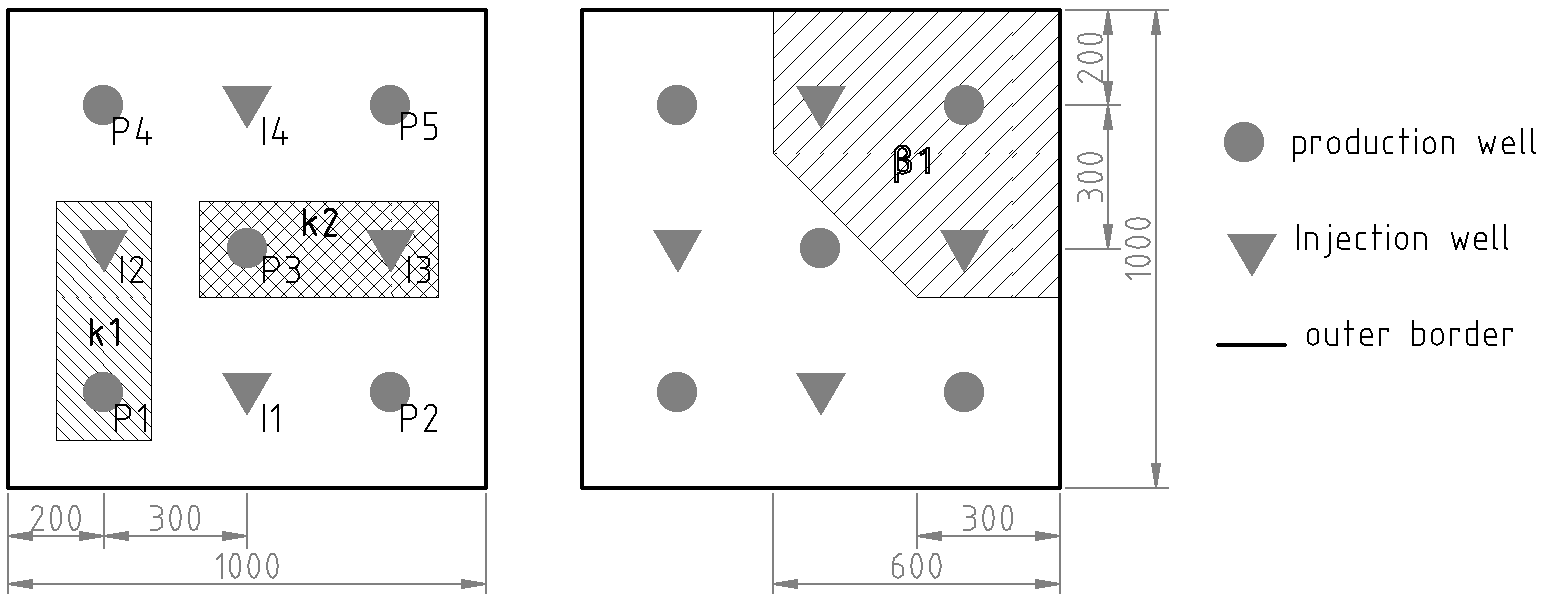
\includegraphics[width=0.7\linewidth]{fig1}
	\caption{Схематичечское представление расчётной области Schematic representation of the computational domain spacing pattern}
	\label{fig:schime}
\end{figure}

В качестве источника исходных данных была использована синтетическая гидродинамическая модель. Набор данных получен путем прямого численного моделирования двухфазной фильтрации воды и нефти. Полученные данные были использованы для решения задачи адаптации и прогнозирования.

При решении обратной задачи в качестве режимов работы использованы дебиты добывающих скважин и приемистости нагнетательных скважин, полученные из прямого численного моделирования. Пористость, толщина пласта, начальные и граничные условия соответствовали прямой задаче. Обратная задача решается в оптимизационной постановке, в которой минимизируется целевая функция {\ref{mse}}. В качестве фактических замеров пластового давления использовалось ограниченное количество давлений, полученные из решения прямой задачи. Случайным образом выбраны 10\% от общего количества значений пластового давления, которые выступали в качестве истинных значений.

Период моделирования составлял 10 лет, на протяжении которых скважины работали с заданными режимами. Расчетный шаг составлял 1 месяц. Зависимости приемистости нагнетательных скважин от времени, приведенные на рис. \ref{fig:fig002}, получены путем случайной генерации и имеют кусочно-постоянный вид. Так же с заданной периодичностью происходит отключение нагнетательных скважин, период простоя составлял от 2 до 4 месяцев. На добывающих скважинах заданы изменяющиеся по гармоническому закону забойные давления, которые приведены на рис. \ref{fig:fig003}.

Полученный набор данных был использован для решения обратной задачи. При этом для оценки прогностических свойств модели данные были разделены на обучающую и тестовую выборки. Первые 7 лет истории разработки отнесены к обучающей выборке и использованы для адаптации модели. Период 7-10 лет включен в тестовую выборку для которой проведены прогнозные расчеты. Тестовая и обучающая выборки обозначены на рис. \ref{fig:fig002} - \ref{fig:fig004} зеленым и красным цветом фона соответственно.

\begin{figure}
	\centering
	\begin{minipage}{0.5\linewidth}
		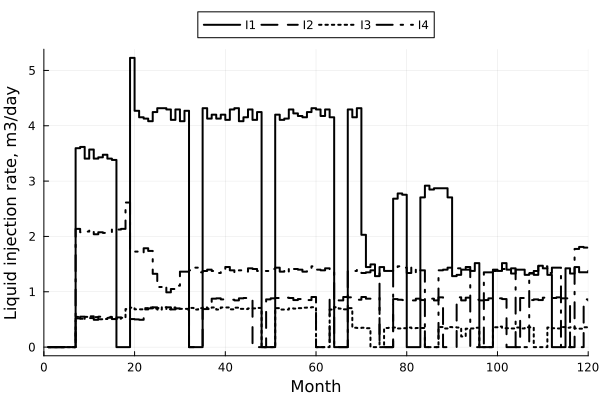
\includegraphics[width=1\textwidth]{fig2a}
		\caption{a}
		\label{inj_rate}
	\end{minipage}%
	\begin{minipage}{0.5\linewidth}
		\centering
		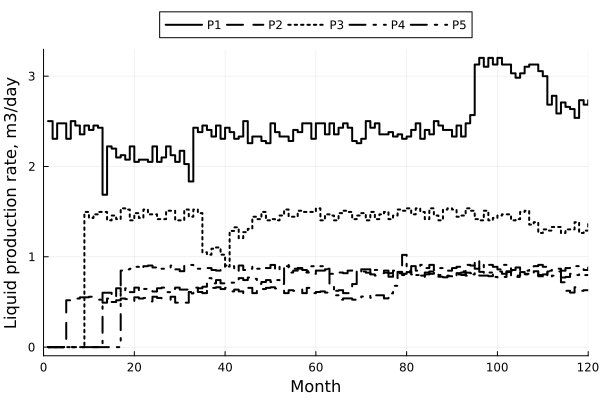
\includegraphics[width=1\textwidth]{fig2b}
		\caption{b}
		\label{prod_rate}
	\end{minipage}
	\caption{Динамика приемистости нагнетательных скважин I1-I4 Injectivity dynamics of injection wells I1-I4}
\end{figure}

 Начальное пластовое давление составляло 20 МПа. На границах элемента разработки задано Постоянное пластовое давление $Pa = 20 MPa$. Параметры горной породы и насыщающих ее флюидов, принятые для расчета, имели следующие значения: пористость 0.2, значения абсолютной проницаемости представлены в виде карты на рис. 1, эффективная вязкость 1 мПа*c. Толщина пласта принята равной 4 м.

Решение оптимизационной задачи осуществляется встроенными в пакет Flux оптимизационными алгоритмами (Descent и ADAM). В результате решения были получены карты подвижности \ref{fig:mob} и карты эффективной сжимаемости \ref{comp}. Несмотря на отличия, видно, что поля качественно повторяют исходные (\ref{fig:schime}). Кроме поля подвижности на \ref{fig:mob} представлены связи между скважинами и их значения, которые были получены методом частичного исключения переменных из численной фильтрационной модели \cite{and}. Наибольшие значения связей 1-7 и 3-8 соответствуют промытым водой высокопроводящим каналам. Коэффициенты связей имеют смысл проводимости между скважинами на единицу толщины пласта. Подобные коэффициенты связи могут быть получены при интерпретации попарного гидропрослушивания скважин.

\begin{figure}
	\centering
	\begin{minipage}{0.5\linewidth}
		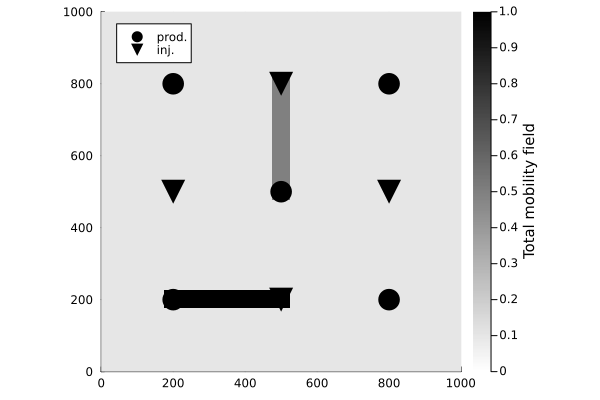
\includegraphics[width=1\textwidth]{fig4}
		\caption{a}
		\label{fig:mob}
	\end{minipage}%
	\begin{minipage}{0.5\linewidth}
		\centering
		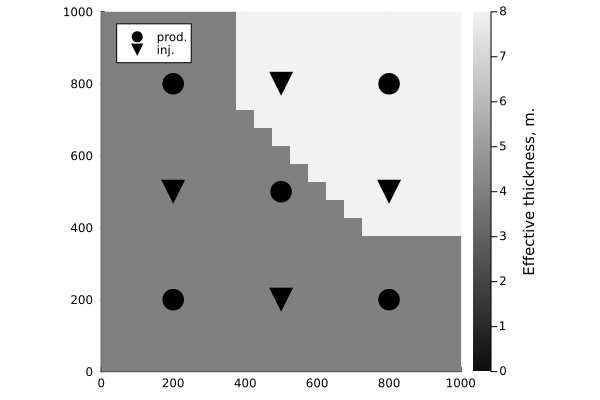
\includegraphics[width=1\textwidth]{fig5}
		\caption{b}
		\label{comp}
	\end{minipage}
	\caption{a Поле общей подвижности на конце обучающей выборки Total mobility field at the end of the training set
	b Восстановленное поле общей подвижности Restored general total field}
\end{figure}


Количественное сопоставление истинного и восстановленного поля общей подвижности проведено на основе рассчитанных для них величин связей между скважинами. Сравнение связей приведено в таблице из которой видно, что ранжирование восстановленных связей полностью совпадает с ранжированием истинных связей. Кроме того, получено удовлетворительное количественное совпадение величин связей: в среднем относительная ошибка составляет 9\%. Таким образом, восстановленное поле общей подвижности качественно и количественно воспроизводит ключевые особенности истинного поля.

\begin{figure}
	\centering
	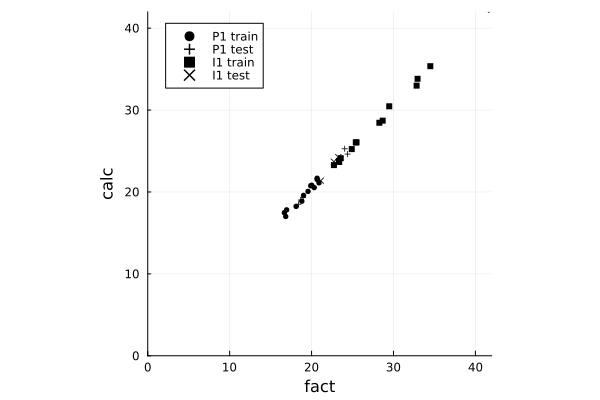
\includegraphics[width=0.7\linewidth]{fig6}
	\caption{Сопоставление фактических и расчетных значений пластового давления для добывающих и нагнетательных скважин. Полые маркеры соответствуют обучающей выборке, закрашенные – тестовой выборке. Пунктирная линия обозначает интервал отклонения в 10\% Comparison of true and calculated values of reservoir pressure for production and injection wells. Hollow markers correspond to the training set, filled markers correspond to the test set. The dotted line indicates the 10\% deviation interval}
	\label{fig:cp}
\end{figure}


Для реальных пластовых систем величины связей между скважинами, как правило, достоверно не известны. В виду этого одним из основных критерием для оценки качества адаптации модели выступают замеры пластового давления. На рис. 8 приведено сравнение значений фактических и расчетных пластовых давлений, полученных после восстановления поля общей подвижности. Полыми маркерами обозначены значения соответствующие обучающей выборке, закрашенными – тестовой. Видно, что получено удовлетворительное совпадение давлений  на обучающей и тестовой выборке, значения средней относительной ошибки для которых составляет 2.6 и 4.1\% соответственно. Модель демонстрирует удовлетворительную точность на тестовой выборке, что подтверждает ее прогнозные свойства.


	\begin{table}[h!]
	\caption{Коэффициенты связей между скважинами}	
	\label{tabl:connection}	
	\begin{center}
		\begin{tabular}{c|c|c|c|c}
			\hline
			Связь & Истинное значение & Восстановленное значение & Относительная ошибка д.ед. \\
			\hline
			1-6 & 0.4 & 15.7 & 0.1 \\
			1-7 & 0.9 & 1.7 & 0.1  \\
			1-3 & 0.5 & 0.7 & 0.1  \\
			4 & 0.5 & 184.9 & 0.1  \\
			5 & 1.9 & 2.2 & 0.2  \\
			6 & 0.9 & 1.8 & 0.1  \\
			7 & 0.7 & 1.7 & 0.1  \\
			8 & 1.1 & 1.8 & 0.1  \\
			9 & 0.9 & 1.0 & 0.1  \\
			\hline
			
		\end{tabular}
	\end{center}
\end{table}


\section{CONCLUSIONS}

Предложен подход к совместному применению теории фильтрации и машинного обучения для адаптации однофазной модели фильтрации на историю разработки. На примере синтетической модели элемента нефтяного месторождения с зонально неоднородным полем проницаемости и эффективной сжимаемости была продемонстрирована реализация предложенных подходов.
Адаптация однофазной модели фильтрации на историю проведена путем восстановления поля общей подвижности и эффективной сжимаемости с помощью сети радиально-базисных функций. На основе восстановленного поля рассчитаны коэффициенты связи между скважинами, которые качественно и количественно соответствуют истинным связям.

\section{FUNDING}
«Исследование выполнено за счет гранта Российского научного фонда № 24-21-00468,
 https://rscf.ru/project/24-21-00468/»

\begin{thebibliography}{20}
	
\bibitem{mus1} Musakaev E. N., Rodionov S. P. Musakaev N. G. 2021. Hierarchical Approach to Identifying Fluid Flow Models in a Heterogeneous Porous Medium // Mathematics. 2021. Vol. 9. No. 24. 3289. https://doi.org/10.3390/math9243289

\bibitem{maz} Mazo A.B., Potashev K. A. 2020. Superelementy. Modelirovanie razrabotki neftyanykh mestorozhdeniy. Moskva: INFRA-M. 219p. [In Russian]

\bibitem{bek} Bekman A. D., Pospelova T. A., Zelenin D. V. 2020. A new approach to water cut forecasting based on results of capacitance resistance modeling // Tyumen State University Herald. Physical and Mathematical Modeling. Oil, Gas, Energy, vol. 6, no. 1 (21), P. 192-207. https://doi.org/10.21684/2411-7978-2020-6-1-192-207 [In Russian]

\bibitem{pot} Potashev K.A., Akhunov R.R., Mazo A.B. 2022. Calculation of the flow rate between wells in the flow model of an oil reservoir using streamlines // Georesources. 24(1), pp. 27–35. https://doi.org/10.18599/grs.2022.1.3 [In Russian]

\bibitem{tem} Temirchev P., Simonov M., Kostoev R., Burnaev E., Oseledets I., Akhmetov A., Margarit A., Sitnikov A., Koroteev D. 2020. Deep neural networks predicting oil movement in a development unit // Journal of Petroleum Science and Engineering. Vol. 184. P. 106513. https://doi.org/10.1016/j.petrol.2019.106513

\bibitem{ill} Illarionov E., Temirchev P., Voloskov D., Kostoev R., Simonov M., Pissarenko D., Orlova D., Koroteev D. 2022. End-to-end neural network approach to 3D reservoir simulation and adaptation // Journal of Petroleum Science and Engineering Vol. 208. P. 109332. https://doi.org/10.1016/j.petrol.2021.109332

\bibitem{uma} Umanovskiy A. W. 2022. Proxy modeling pf reservoir hydrodynamics with graph neural networks // Tyumen State University Herald. Physical and Mathematical Modeling. Oil, Gas, Energy. Vol 8. No 3 (31). P. 155-177. https://doi.org/10.21684/2411-7978-2022-8-3-155-177 [In Russian]

\bibitem{gop} Gopa K., Yamov S., Naugolnov M., Perets D., Simonov M. 2018. Cognitive Analytical System Based on Data-Driven Approach for Mature Reservoir Management // SPE Russian Petroleum Technology Conference (October 15, 2018, Moscow, Russia). https://doi.org/10.2118/191592-18RPTC-MS

\bibitem{kos1} Kosyakov V. P., Legostaev D. Yu., Musakaev E. N. 2021. The problem of the combined use of filtration theory and machine learning elements for solving the inverse problem of restoring the hydraulic conductivity of an oil field // Tyumen State University Herald. Physical and Mathematical Modeling. Oil, Gas, Energy. Vol. 7. No. 2 (26). P. 113-129. https://doi.org/10.21684/2411-7978-2021-7-2-113-129 [In Russian]

\bibitem{kos2} Kosyakov V. P., Legostaev D. Yu. 2022. Using elements of machine learning to solve the inverse problem of reconstructing the hydraulic conductivity feld for a filtration problem // Tyumen State University Herald. Physical and Mathematical Modeling. Oil, Gas, Energy. Vol. 8. No. 2 (30). P. 129-149. https://doi.org/10.21684/2411-7978-2022-8-2-129-149 [In Russian]

\bibitem{kos3} Kosyakov V. P., Rodionov S. P. 2016. Оптимальное управление системой скважин на основе уравнений двухфазной фильтрации	Труды МФТИ – 2016. – Том 8. – №3(31) – С. 79–90. ISSN 2072-6759

\bibitem{far} Farrell P. E., Ham D. A., Funke S. W., Rognes M. E. 2013. Automated Derivation of the Adjoint of High-Level Transient Finite Element Programs // SIAM Journal on Scientific Computing. Vol. 35. No. 4. P. C369-C393. https://doi.org/10.48550/arXiv.1204.5577

\bibitem{inn} Innes M.,  Saba E, Fischer K., Gandhi D., Rudilosso M.C., Joy N.M., Karmali T., Pal A. 2018. Fashionable Modelling with Flux // Viral Shah // ArXiv. https://doi.org/10.48550/arXiv.1811.01457 

\bibitem{and} Andreev V.B. 2013. Numerical methods. М.: MAKS Press. 336 p.

\bibitem{hor} Horchreiter S., Schmidhuber S. 1997. Long short-term memory // Neural computation Neural Computation. Vol. 9. P. 1735-80. https://doi.org/10.1162/neco.1997.9.8.1735


\bibitem{mus} E.N.Musakaev, S.P.Rodionov, D.Y.Legostaev, V.P.Kosyakov, "Parameter identification for sector filtration model of an oil reservoir with complex structure" // AIP Conference Proceedings 2125,030113 2019;

\bibitem{kos} V. P. Kosyakov. "Structural and Parametric Identification of an Aquifer Model for an Oil Reservoir". Lobachevskii J Math. 2020. V. 41, P. 1242-1247.

\bibitem{bas} K. S. Basniev, N. M. Dmitriev, R. D. Kanevskaya, V. M. Maksimov. \textit{Underground hydromechanics}. M.-Izhevsk: Institute for Computer Research, 2006. [in Russian]

\bibitem{azi} H. Aziz, E. Settari. \textit{Mathematical modeling of reservoir systems}.  M.-Izhevsk: Institute for Computer Research, 2004. [in Russian]

\bibitem{opt} V.P.Kosyakov, S.P.Rodionov "Optimal control of wells on the basis of two-phase filtration equations". Proceedings of MIPT. 2016. V. 8, N 3. P. 79-90.

\bibitem{leg} V. P. Kosyakov,  D. Yu. Legostaev. "Using elements of machine learning to
solve the inverse problem of reconstructing the hydraulic conductivity feld for a fltration
problem". Tyumen State University Herald. Physical and Mathematical Modeling. Oil, Gas,
Energy, V. 8, N 2 (30), P. 129-149.

\end{thebibliography}

\end{document}
